%% Packages indispensables
\documentclass[a4paper, 12pt]{article}
\usepackage[utf8]{inputenc}
\usepackage[T1]{fontenc}
\usepackage[francais]{babel}

\usepackage[a4paper]{geometry}
\usepackage{graphicx}

\newcommand{\package}[1]{\texttt{#1}}
\newcommand{\kv}[2]{\textit{<#1>}\texttt=\textit{<#2>}}
\newcommand{\key}[3]{\textbf{\texttt{#1} (valeur par défaut : \texttt{#2})} #3}
\newcommand{\commande}[1]{\texttt{\textbackslash#1}}


\usepackage{hyperref}
\hypersetup{
	colorlinks=true,
	linkcolor=blue,
	urlcolor=blue,
}

\title{Package \texttt{playcards.sty} pour \LaTeX}
\date{\today}
\author{Clément \bsc{Pagès} \texttt{contact -- arobase -- clementpages point fr}}

\begin{document}
\maketitle

Ce petit package fournit des commandes pour dessiner des cartes à jouer, de largeur 59 mm et de hauteur 89 mm. Ce sont les dimensions des cartes classiques.

\tableofcontents

\section*{Remerciements}
Je remercie Christophe \bsc{Poulain} pour son génial package \href{https://ctan.org/pkg/profcollege}{ProfCollege}, dont le code m'a servi d'inspiration pour la syntaxe des commandes utilisées ici. Et plus globalement pour ce package exceptionnel, devenu indispensable !

Merci également à \href{https://tex.stackexchange.com/users/1948/didest}{didest}, dont la question posée sur \href{https://tex.stackexchange.com/questions/47924/creating-playing-cards-using-tikz}{StackExchange} m'a servi de base.

\section{Téléchargement, installation, prérequis}
Le package est disponible sur CTAN : \href{https://ctan.org/pkg/playcards}{https://ctan.org/pkg/playcards}. Il contient un unique fichier : \texttt{playcards.sty}.

Certains packages sont chargés automatiquement. Ils sont installés par défaut sur la majorités des installations classiques :
\begin{description}
	\item[\package{tikz}] et certaines de ses librairies.
	\item[\package{simplekv}] pour gérer les paramètres facultatifs des commandes par système \kv{clé}{valeur}.
	\item[\package{graphicx}] pour les images. 
	\item[\package{contour}] pour les ombres et contours de textes.
	\item[\package{geometry}] configuré pour optimiser l'occupation d'une feuille A4 en la remplissant de cartes convenablement alignées.
\end{description}

\section{Principe général}
Les principales commandes sont construites sur un système de clés/valeurs, sur le modèle \texttt{\textbackslash commande[\kv{cle1}{valeur1}, \kv{cle2}{valeur2}, …]\{param1\}\{param2\}}.

Toutes les clés sont facultatives et si elles ne sont pas renseignées, il leur est attribué une valeur par défaut.

Sauf précision contraire, les longueurs sont mentionnées en millimètres.

\section{Commandes fournies}
	\subsection{Commande \commande{drawcardsrecto}}
Cette commande prend un paramètre obligatoire : le texte qui apparaîtra au centre de la carte. Elle remplit une feuille A4 avec 9 cartes identiques. Cette commande trace le recto des cartes. Un exemple est donné figure \ref{fig:recto}.
\begin{figure}[h]\begin{center}
	\caption{\commande{drawcardsrecto[trame=false]\{5\}}}
	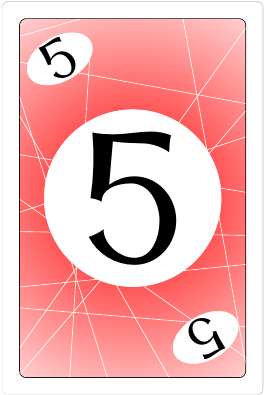
\includegraphics{screen01.png}\label{fig:recto}
\end{center}\end{figure}

Paramètres optionnels :
\begin{itemize}
	\item \key{borders}{true}{Trace les bordures. Si \texttt{false}, les bordures sont retirées.}
	\item \key{trame}{true}{Si \texttt{true}, remplit une feuille A4 avec les cartes. Si \texttt{false}, dessine une seule carte.}
	\item \key{corners}{true}{Si \texttt{true}, le texte de la carte est reporté à l'endroit à et à l'envers dans les coins. Si \texttt{false}, les coins ne sont pas affichés.}
	\item \key{backgroundImg}{true}{Si \texttt{true}, affiche l'arrière-plan. Si \texttt{false}, pas d'arrière-plan.}
	\item \key{backgroundColor}{red}{Spécifie la couleur de l'arrière-plan. Sera ignoré si \texttt{backgroundImg=false}. Utilise les couleurs du package \href{https://www.ctan.org/pkg/xcolor}{xcolor}.}
	\item \key{contentsFontSize}{120}{Taille (en pt) du texte au centre de la carte.}
	\item \key{cicleRay}{20}{Rayon du cercle blanc au centre de la carte. La valeur \texttt 0 équivaut à ne pas tracer le cercle.}
\end{itemize}

	\subsection{Commande \commande{drawcardsverso}}
Il est possible, mais ce n'est pas obligatoire, de dessiner le verso des cartes. Les rectos devront être sur une page et les versos sur une autre. Il est recommandé d'avoir autant de rectos que de versos pour préserver l'alignement. Un exemple est donné figure \ref{fig:verso}.

Pour avoir le bon alignement, il est recommandé de placer les commandes dans un environnement \verb!\begin{center}...\end{center}!.
\begin{figure}[h]\begin{center}
	\caption{\commande{drawcardsverso[trame=false,contentsFontSize=40]\{Exemple\}}}
	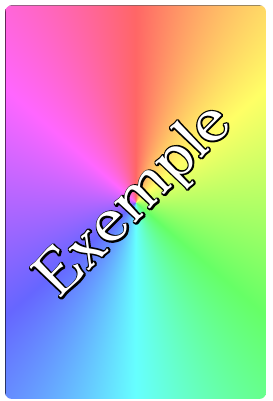
\includegraphics{screen02.png}\label{fig:verso}
\end{center}\end{figure}

Paramètres optionnels :
\begin{itemize}
	\item \key{backgroundImg}{true}{Si \texttt{true}, affiche l'arrière-plan. Si \texttt{false}, pas d'arrière-plan.}
	\item \key{trame}{true}{Si \texttt{true}, remplit une feuille A4 avec les cartes. Si \texttt{false}, dessine une seule carte.}
	\item \key{contentsFontSize}{50}{Taille (en pt) du texte au centre de la carte.}
\end{itemize}

\end{document}
